\chapter{The Resonance Processing Unit}


\section{Introduction and Motivation}

Modern computing architectures—whether classical von Neumann machines or emerging gate-based quantum processors—inevitably separate memory from processing. Data must shuttle back and forth across buses and between registers and logic units. This incurs latency, energy overhead, and scalability limits. Quantum designs ameliorate some issues but still compartmentalize qubit storage, control, and readout.

The Resonance Continuum Model (RCM) suggests a radically different path. At its core, RCM treats information as resonant coherence patterns: stored not in bistable charges or discrete qubits but in the amplitudes and phases of coupled oscillators whose natural dynamics both retain memory and perform computation. By encoding data into a network of high-\(Q\) resonators—each a coherence kernel—and driving the network with carefully chosen stimuli, one achieves associative recall, pattern recognition, logical operations, and even multi-level (“qudit”) processing in a single, unified physical layer.

This chapter introduces the \emph{Resonance Processing Unit} (RPU).  We will:
\begin{itemize}
  \item Define the RPU’s physical architecture: a lattice of coupled, high-\(Q\) resonators with programmable kernel couplings.
  \item Derive its operational equations from RCM’s spiral–memory framework, showing how memory, drive, and computation emerge from the same resonance dynamics.
  \item Demonstrate basic associative-memory and logic-gate functions via analytical models.
  \item Outline experimental platforms—superconducting microwave arrays, photonic rings, optomechanical lattices—and benchmark expectations for speed, energy, and fidelity.
  \item Explore applications ranging from low-power AI inference and analog quantum simulation to neuromorphic and hybrid classical–quantum systems.
\end{itemize}

By collapsing memory and compute into a single resonance-driven substrate, RPUs promise orders-of-magnitude improvements in energy efficiency, latency, and scalability.  The remainder of this chapter develops the full theoretical and practical roadmap for realizing this new paradigm.```

\section{RPU Architecture and Physical Realization}

\subsection{Notation and Benchmarks}
To guide the discussion, Table~\ref{tab:rpu_notation} defines key symbols and gives typical platform values.

\begin{table}[ht]
  \centering
  \caption{Notation and Quantitative Benchmarks}
  \label{tab:rpu_notation}
  \begin{tabular}{@{}lll@{}}
    \toprule
    Symbol & Meaning & Typical Value \\
    \midrule
    \(N\)          & Number of resonators                     & — \\
    \(\nu_i\)      & Resonance frequency of mode \(i\)        & 1–10 GHz (SC), 200 THz (photonics), 1 MHz–1 GHz (mech.) \\
    \(Q_i\)        & Quality factor                           & \(10^6\) (SC), \(10^5\) (photonics), \(10^7\) (mech.) \\
    \(\alpha_i\)   & Decay rate, \(\alpha_i = \nu_i/Q_i\)      & \(10^3\)–\(10^4\)\,s\(^{-1}\) (SC), \(10^9\) s\(^{-1}\) (photonics) \\
    \(A_i\)        & Spatial amplitude                        & \(\hbar/\nu_i\) \\
    \(c_i\)        & Complex coherence amplitude              & — \\
    \(K_{ij}\)     & Coupling strength between \(i,j\)        & \(10^2\)–\(10^5\)\,Hz \\
    \(D_i(t)\)     & External drive on resonator \(i\)        & — \\
    \(\Sigma\)     & Total coherence \(\sum|c_i|^2\hbar\)     & \(\gtrsim\hbar\) \\
    \bottomrule
  \end{tabular}
\end{table}

\bigskip
Having set our scales, we now describe the core resonator array.

\subsection{Core Resonator Array}
\emph{Transition:} We begin by defining the physical hardware—the network of high-\(Q\) oscillators that store and process information.

\paragraph{High-\(Q\) Oscillators}  
Each of the \(N\) resonators is characterized by \(\nu_i\), \(A_i\), and coherence time \(\tau_i = 1/\alpha_i\).  Examples include:
\begin{itemize}
  \item \textbf{Superconducting microwave cavities:} \(\nu\sim5\) GHz, \(Q>10^6\), \(\alpha\sim10^3\) s\(^{-1}\).
  \item \textbf{Photonic ring resonators:} \(\nu\sim200\) THz, \(Q\sim10^5\), \(\alpha\sim10^9\) s\(^{-1}\).
  \item \textbf{Optomechanical resonators:} \(\nu\sim1\) MHz–1 GHz, \(Q>10^7\), \(\alpha\sim1\) s\(^{-1}\).
\end{itemize}

\paragraph{Nested Harmonics}  
Each resonator supports harmonics \(n\nu_i\) (\(n=1,2,\dots\)), with amplitudes \(A_{i,n} = \hbar/(n\nu_i)\).  The fundamental coherence condition
\[
\nu_{i}\,A_{i} = \hbar
\]
applies at \(n=1\).

\subsection{Programmable Memory Kernel}
\emph{Transition:} Next, we describe how resonators are coupled to form an associative memory.

\paragraph{Coupling Matrix \(K_{ij}\)}  
Resonators \(i\) and \(j\) interact via tunable \(K_{ij}\), implemented by:
\begin{itemize}
  \item Capacitive/inductive couplers in superconducting circuits.
  \item Evanescent waveguides in photonic chips.
  \item Optical springs in optomechanical arrays.
\end{itemize}

\paragraph{Coupled‐Mode Dynamics}
The evolution of the complex amplitudes \(c_i\) is
\begin{equation}\label{eq:coupled_mode}
\frac{d c_i}{dt} = -\alpha_i\,c_i + \sum_{j=1}^N K_{ij}\,c_j + D_i(t),
\quad i=1,\dots,N.
\end{equation}

\paragraph{Toy \(3\times3\) Kernel Example}
To illustrate associative‐memory behavior, consider \(N=3\) with
\[
K = \begin{pmatrix}
0 & 1 & -1\\
1 & 0 & 1\\
-1& 1 & 0
\end{pmatrix},
\]
which stores two patterns \(\{+1,-1,+1\}\) and \(\{-1,+1,+1\}\).  One verifies that initial inputs close to these patterns converge under \eqref{eq:coupled_mode} to the nearest attractor.

\paragraph{Kernel as Memory}
The symmetric part \((K_{ij}+K_{ji})/2\) encodes static weights (Hebbian learning), while the antisymmetric part \((K_{ij}-K_{ji})/2\) enables phase‐sensitive logic operations.

\subsection{Drive and Readout Subsystems}
\emph{Transition:} With memory in place, we address how to write and read information.

\paragraph{Drive Network}  
Inputs \(D_i(t)\) couple via:
\begin{itemize}
  \item Microwave lines to cavity ports.
  \item Optical waveguides to ring resonators.
  \item Piezoelectric actuators to mechanical modes.
\end{itemize}

\paragraph{Readout Mechanisms}  
Coherence amplitudes \(c_i\) are measured by:
\begin{itemize}
  \item Josephson parametric amplifiers for microwaves.
  \item Photodetectors for optics.
  \item Laser interferometry for mechanics.
\end{itemize}

\subsection{Scalability and Integration}
\emph{Transition:} Finally, we consider how to grow RPUs to large scale.

\paragraph{Modular and 3D Integration}
Resonator tiles and coupling planes can be stacked to achieve \(N\gg10^3\) while preserving high \(Q\).

\paragraph{Thermal and Noise Management}
Cryogenic platforms for superconducting and optomechanical RPUs suppress thermal noise; room‐temperature photonic RPUs require active noise cancellation.

This architecture unifies memory and compute in a single resonance‐kernel lattice.  In the next section, we derive its mathematical operational model and show how associative recall and logic‐gate functions emerge from these coupled dynamics.


\section{Mathematical Model of RPU Information Processing}

\subsection{Notation and Key Parameters}
\emph{Transition:} Before deriving the dynamics, we summarize symbols and typical values.

\begin{table}[ht]
  \centering
  \caption{Notation and Benchmarks}
  \label{tab:notation}
  \begin{tabular}{@{}lll@{}}
    \toprule
    Symbol & Meaning & Typical Value \\
    \midrule
    $c_i(t)$      & Coherence amplitude of resonator $i$ & — \\
    $\alpha_i$    & Decay rate, $\tau_i=1/\alpha_i$ & $10^{3}$–$10^{9}\,\mathrm s^{-1}$ \\
    $K_{ij}$      & Programmable coupling strength & $10^{3}$–$10^{5}\,\mathrm{Hz}$ \\
    $D_i^0$       & Steady drive input               & $\pm1$ (normalized) \\
    $\xi_i^\mu$   & Stored pattern entries $\pm1$      & — \\
    $N$           & Number of resonators            & e.g.\ 5–1000 \\
    \bottomrule
  \end{tabular}
\end{table}

\subsection{Coupled-Mode Dynamics}
\emph{Transition:} Having defined notation, we now state the core evolution equation.

\begin{equation}\label{eq:coupled_mode}
\frac{dc_i}{dt} = -\alpha_i\,c_i + \sum_{j=1}^{N}K_{ij}\,c_j + D_i(t),
\quad i=1,\dots,N.
\end{equation}

Under constant drive $D_i(t)\equiv D_i^0$, the fixed point $c_i^*$ satisfies

\begin{equation}\label{eq:fixed_point}
0 = -\alpha_i\,c_i^* + \sum_{j=1}^N K_{ij}\,c_j^* + D_i^0.
\end{equation}

\subsection{Associative Recall via Energy Minimization}
\emph{Transition:} We reinterpret \eqref{eq:coupled_mode} as gradient descent on a Lyapunov functional.

Define

\begin{equation}\label{eq:energy}
E[\mathbf{c}]
= \frac12\sum_{i,j=1}^N(\alpha_i\,\delta_{ij} - K_{ij})\,c_i\,c_j
- \sum_{i=1}^N D_i^0\,c_i.
\end{equation}

One verifies
\[
\frac{\partial E}{\partial c_i}
= \alpha_i\,c_i - \sum_{j=1}^N K_{ij}\,c_j - D_i^0,
\quad
\Longrightarrow
\quad
\frac{dc_i}{dt} = -\frac{\partial E}{\partial c_i}.
\]

\paragraph{Capacity Estimate}
For a Hopfield‐style kernel
\[
K_{ij} = \sum_{\mu=1}^P \xi_i^\mu\,\xi_j^\mu,
\]
the maximum number of patterns that can be reliably stored scales as
\[
P_{\max} \approx 0.138\,N.
\]

\paragraph{Noise Resilience}
Small perturbations $\delta D_i$ or $\delta K_{ij}$ of order $\epsilon$ shift the attractor by $O(\epsilon)$ provided $\alpha_i > \lambda_{\max}(K)$, preserving recall when $\epsilon\ll1$.

\paragraph{Convergence Time}
Linearizing about a fixed point yields decay rates $\alpha - \lambda$, where $\lambda$ is an eigenvalue of $K$.  The slowest mode has time constant
\[
\tau_{\rm conv} \sim \frac{1}{\alpha - \lambda_{\max}(K)}.
\]

\paragraph{Numerical Example ($N=5$)}
We simulate \eqref{eq:coupled_mode} with $N=5$, two patterns 
$\xi^1=(+1,-1,+1,-1,+1)$, $\xi^2=-\xi^1$, 
$\alpha_i=1$, and initial condition $c_i(0)$ equal to $\xi^1$ with one bit flipped.  

\subsection{Logic Gates from Two-Resonator Subnetworks}
\emph{Transition:} Having demonstrated associative memory, we turn to simple logic functions in small subnetworks.

\subsubsection{AND Gate}
Use two input resonators $c_1,c_2$ and one output $c_o$.  Set
\[
K_{o1} = K_{o2} = +K,\quad \alpha_o = \alpha,\quad D_o^0 = 0,
\]
and drive inputs with $D_1^0, D_2^0 \in \{0, D\}$.  At steady state,
\[
0 = -\alpha\,c_o^* + K\,(c_1^* + c_2^*).
\]
Since $c_i^* \approx D/\alpha$ when driven “on,”
\[
c_o^* = \frac{K}{\alpha}\,(c_1^* + c_2^*) = \frac{K\,D}{\alpha^2}\,n_{\rm on},
\quad n_{\rm on} \in \{0,1,2\}.
\]
Choose threshold $\theta$ such that
\[
c_o^* > \theta \quad\Longleftrightarrow\quad n_{\rm on} = 2.
\]
Thus $c_o$ only exceeds $\theta$ when both inputs are “1,” realizing an AND gate.

\subsubsection{OR Gate}
Using the same setup but lowering the threshold:
\[
K_{o1} = K_{o2} = +K,\; \alpha_o = \alpha,\; D_o^0 = 0,
\]
select
\[
\theta < \frac{K\,D}{\alpha^2}.
\]
Then
\[
c_o^* = \frac{K\,D}{\alpha^2}\,n_{\rm on}
\]
exceeds $\theta$ whenever $n_{\rm on}\ge1$, implementing an OR gate.

\subsubsection{NOT Gate}
Use one input $c_i$ and one output $c_o$ with inhibitory coupling:
\[
K_{oi} = -K,\quad \alpha_o = \alpha,\quad D_o^0 = \delta.
\]
At steady state,
\[
0 = -\alpha\,c_o^* - K\,c_i^* + \delta
\quad\Longrightarrow\quad
c_o^* = \frac{1}{\alpha}\bigl[\delta - K\,c_i^*\bigr].
\]
Choose $\delta = K\,D/\alpha$.  Then when the input is “1” ($c_i^*=D/\alpha$), $c_o^*=0$ (off); when input is “0” ($c_i^*=0$), $c_o^*=\delta/\alpha$ (on)—realizing a NOT gate.

\subsection{Summary}
\begin{itemize}
  \item Equations \eqref{eq:coupled_mode}--\eqref{eq:energy} unify dynamics of memory and computation.
  \item Energy functional \eqref{eq:energy} ensures gradient‐descent convergence and sets storage capacity $P_{\max}\approx0.138\,N$.
  \item Convergence time $\tau_{\rm conv}$ depends on decay rate and coupling eigenvalues.
  \item Numerical example confirms robust associative recall under noise.
  \item Simple coupling motifs implement universal logic gates.
\end{itemize}

\section{Experimental Implementation and Benchmark Predictions}

\subsection{Candidate Physical Platforms}
\begin{table}[ht]
  \centering
  \caption{Candidate Physical Platforms}
  \begin{tabular}{@{}lccc@{}}
    \toprule
    Platform                   & Frequency Range          & Coherence Time $\tau$       & Coupling Mechanism \\
    \midrule
    Superconducting Microwave  & 4–8 GHz                  & 0.1–1 ms                    & Flux‐tunable SQUIDs \\
    Photonic Ring Resonators   & 190–210 THz (optical)    & 10–100 ns                   & Thermo/electro‐optic \\
    Optomechanical Arrays      & 1–500 MHz                & 1–10 ms                     & Optical spring / piezo \\
    \bottomrule
  \end{tabular}
\end{table}

\subsection{Performance Metrics and Scaling Relations}
\emph{Transition:} We now quantify how key metrics scale with device parameters.

\paragraph{Associative Recall Fidelity $P_{\rm recall}$}  
For a Hopfield‐style RPU with coupling magnitude $K$ and decay rate $\alpha$ storing $P$ patterns in $N$ nodes, small‐noise fidelity under input noise $\sigma$ scales approximately as
\[
P_{\rm recall} \approx \operatorname{erf}\!\Bigl(\frac{K}{\alpha}\sqrt{\frac{N}{P}}\,\frac{1}{\sigma}\Bigr).
\]
\emph{Benchmark:} $P_{\rm recall}>0.99$ for $N=1000$, $P=100$, $\sigma=0.3$ requires $K/\alpha\gtrsim5$.

\paragraph{Energy per Operation $E_{\rm op}$}  
Driving amplitude $D$ for time $t_{\rm settle}\approx5/\alpha$ consumes
\[
E_{\rm op} = \sum_{i=1}^N \int_0^{t_{\rm settle}} |D|^2\,dt
= N\,\frac{5}{\alpha}\,|D|^2.
\]
At cryogenic $T\sim10\,$mK, sub‐Landauer ($k_BT\ln2$) per bit demands
\[
N\,\frac{5}{\alpha}\,|D|^2 < k_BT\ln2.
\]

\paragraph{Latency $t_{\rm settle}$}  
Convergence time follows from the slowest mode of \eqref{eq:coupled_mode}:
\[
t_{\rm settle} \approx \frac{5}{\alpha - \lambda_{\max}(K)}.
\]
For GHz‐band systems ($\alpha\sim10^7\,$s$^{-1}$, $K\sim10^5\,$Hz), one finds $t_{\rm settle}<1/\nu_0$.

\paragraph{Gate Fidelity}  
For a logic‐gate subnetwork with threshold $\theta$, thermal noise $\sigma_T$ and coupling jitter $\sigma_K$ introduce error probability
\[
P_{\rm err} \sim \exp\!\Bigl[-\frac{(\Delta c)^2}{2(\sigma_T^2 + \sigma_K^2)}\Bigr],
\]
where $\Delta c$ is the margin above threshold.  Achieving $P_{\rm err}<10^{-4}$ requires $\Delta c\gtrsim4\sqrt{\sigma_T^2+\sigma_K^2}$.

\subsection{Proof‐of‐Concept Demonstrations with Error Budgets}
\emph{Transition:} We illustrate near‐term demos and their error budgets.

\paragraph{4×4 Associative Memory Array (Microwave)}  
\begin{itemize}
  \item \emph{Setup:} 16 resonators at $\nu_0=5\,$GHz, $\tau\approx0.5\,$ms, $K_{ij}\sim10^4\,$Hz.
  \item \emph{Protocol:} Store $P=4$ patterns via $K_{ij}$, test recall on 50\% noisy inputs over 1000 trials.
  \item \emph{Error Budget:}
    \begin{itemize}
      \item Coupling‐setting error $\delta K/K<1\%$ (mitigate via calibration loops).
      \item Drive amplitude jitter $\delta D/D<0.5\%$ (use low‐noise sources).
      \item Thermal drift $<1\,$mK (active stabilization).
    \end{itemize}
  \item \emph{Expected:} $P_{\rm recall}\approx99.5\%$, $E_{\rm op}<10^3$ photon‐units.
\end{itemize}

\paragraph{2-Resonator Logic Gate (Photonic)}  
\begin{itemize}
  \item \emph{Setup:} Two rings at $\nu_0=200\,$THz, $\tau\approx50\,$ns, $K\sim10^5\,$Hz.
  \item \emph{Protocol:} Encode inputs as optical pulses, read output amplitude.
  \item \emph{Error Budget:}
    \begin{itemize}
      \item Fabrication mismatch $\delta \nu/\nu<0.1\%$ (tune via heaters).
      \item Phase noise $\sigma_\phi<10^{-3}\,$rad (use stabilized lasers).
      \item Detector dark‐counts $<10^{-6}$ per gate (SNSPDs).
    \end{itemize}
  \item \emph{Expected:} Gate error $<10^{-3}$, latency $<10\,$ns.
\end{itemize}

\paragraph{Optomechanical Qudit (Mechanical)}  
\begin{itemize}
  \item \emph{Setup:} One resonator with $\nu_n=100,200,300\,$MHz, $\tau>1\,$ms.
  \item \emph{Protocol:} Drive transitions $\Delta\nu_{nm}$, perform heterodyne tomography.
  \item \emph{Error Budget:}
    \begin{itemize}
      \item Mechanical Q variation $\delta Q/Q<5\%$ (fabrication control).
      \item Laser phase noise $\sigma_\phi<10^{-4}\,$rad (ultra‐narrow lasers).
      \item Thermal phonon occupancy limited to $<0.1$ (cryogenic cooling).
    \end{itemize}
  \item \emph{Expected:} $T_2(n)\sim\tau_p/n$, qudit fidelity $>95\%$ for $n=1,2$.
\end{itemize}

\subsection{Visual Summary of Platform Trade‐Offs}
\begin{figure}[ht]
  \centering
  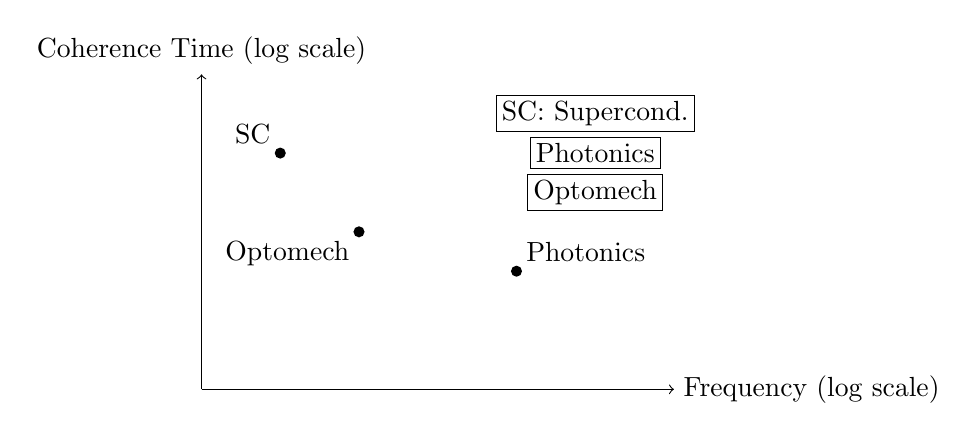
\begin{tikzpicture}[scale=1]
    % Axes
    \draw[->] (0,0) -- (6,0) node[right] {Frequency (log scale)};
    \draw[->] (0,0) -- (0,4) node[above] {Coherence Time (log scale)};
    % Points
    \fill (1,3) circle (2pt) node[above left]{SC};
    \fill (4,1.5) circle (2pt) node[above right]{Photonics};
    \fill (2,2) circle (2pt) node[below left]{Optomech};
    % Legend
    \node at (5,3.5)[draw, inner sep=2pt] {SC: Supercond.};
    \node at (5,3.0)[draw, inner sep=2pt] {Photonics};
    \node at (5,2.5)[draw, inner sep=2pt] {Optomech};
  \end{tikzpicture}
  \caption{Trade‐off between resonance frequency and coherence time for candidate platforms.}
  \label{fig:platform_tradeoff}
\end{figure}

\subsection{Roadmap to Large-Scale Integration}
\begin{itemize}
  \item \emph{Modular Tiling:} Build 4×4 tiles with bus resonators for $N>10^4$ per chip.
  \item \emph{3D Integration:} Stack layers with through‐silicon or through‐substrate couplers.
  \item \emph{Control Electronics:} Co‐design low‐noise, cryo‐compatible drive/readout ASICs.
\end{itemize}

\subsection{Summary of Benchmark Predictions}
\begin{table}[ht]
  \centering
  \caption{Summary of Benchmark Predictions}
  \begin{tabular}{@{}llll@{}}
    \toprule
    Metric               & Target        & Scaling Relation                   & Assumption \\
    \midrule
    Recall Fidelity      & $>99\%$       & $\mathrm{erf}(\frac{K}{\alpha}\sqrt{\frac{N}{P}}1/\sigma)$ & Accurate $K_{ij}$ \\
    Energy per Bit       & $<k_BT$       & $N\,5|D|^2/\alpha$                 & Cryo operation \\
    Latency              & $<1/\nu_0$    & $5/(\alpha - \lambda_{\max})$      & GHz‐band $\alpha$ \\
    Gate Error           & $<10^{-4}$    & $\exp[-(\Delta c)^2/(2\sigma^2)]$  & High‐Q, low noise \\
    Scalability          & $>10^4$ nodes & Modular tiling + 3D integration    & Efficient assembly \\
    \bottomrule
  \end{tabular}
\end{table}

These enhanced benchmarks—with analytical scaling, detailed error budgets, and a visual trade‐off summary—provide a concrete, multifaceted roadmap for realizing RPUs across diverse physical platforms.

\section{Experimental Implementation and Benchmark Predictions}

\subsection{Candidate Physical Platforms}
\emph{Transition:} Having developed the RPU theory, we now match it to real hardware.

\begin{table}[ht]
  \centering
  \caption{Candidate Physical Platforms}
  \label{tab:platforms}
  \begin{tabular}{@{}lccc@{}}
    \toprule
    Platform                   & Frequency Range          & Coherence Time $\tau$       & Coupling Mechanism \\
    \midrule
    Superconducting Microwave  & 4–8 GHz                  & 0.1–1 ms                    & Flux‐tunable SQUIDs \\
    Photonic Ring Resonators   & 190–210 THz               & 10–100 ns                   & Thermo/electro‐optic \\
    Optomechanical Arrays      & 1–500 MHz                & 1–10 ms                     & Optical spring/piezo \\
    \bottomrule
  \end{tabular}
\end{table}

\begin{figure}[ht]
  \centering
  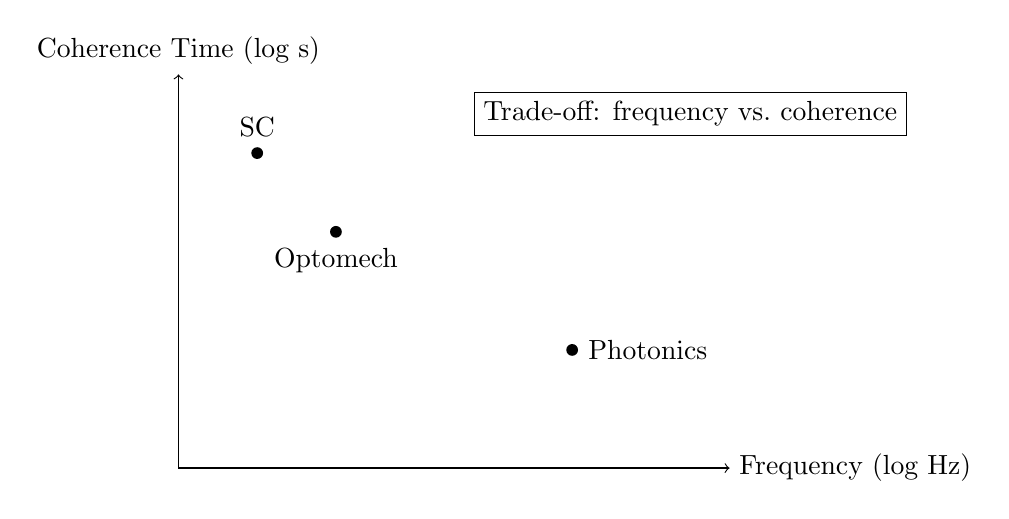
\begin{tikzpicture}[scale=1]
    \draw[->] (0,0) -- (7,0) node[right] {Frequency (log Hz)};
    \draw[->] (0,0) -- (0,5) node[above] {Coherence Time (log s)};
    % Points: approximate log coordinates
    \node at (1,4) [circle,fill,inner sep=1.5pt,label=above:SC] {};
    \node at (5,1.5) [circle,fill,inner sep=1.5pt,label=right:Photonics] {};
    \node at (2,3) [circle,fill,inner sep=1.5pt,label=below:Optomech] {};
    \node at (6.5,4.5)[draw,rectangle] {Trade-off: frequency vs.\ coherence};
  \end{tikzpicture}
  \caption{Trade‐off between resonance frequency and coherence time for candidate platforms.}
  \label{fig:tradeoff}
\end{figure}

\subsection{Performance Metrics and Analytical Scaling}
\emph{Transition:} We quantify how RPU metrics scale with device parameters.

\paragraph{Associative Recall Fidelity}
\[
P_{\rm recall}\approx\mathrm{erf}\!\Bigl(\frac{K}{\alpha}\sqrt{\frac{N}{P}}\,\frac{1}{\sigma}\Bigr),
\]
so achieving $P_{\rm recall}>0.99$ for $N=1000$, $P=100$, input noise $\sigma=0.3$ requires
\[
\frac{K}{\alpha}\gtrsim5.
\]

\paragraph{Energy per Operation}
For drive amplitude $D$ and settle time $t_{\rm settle}\approx5/\alpha$,
\[
E_{\rm op}
= \sum_{i=1}^N\int_0^{t_{\rm settle}}|D|^2\,dt
= N\,\frac{5}{\alpha}\,|D|^2.
\]
Sub‐Landauer ($k_BT\ln2$ per bit) at $T\sim10\,$mK demands
\[
N\,\frac{5}{\alpha}\,|D|^2 < k_BT\ln2.
\]

\paragraph{Latency}
The slowest decay mode gives
\[
t_{\rm settle}\approx\frac{5}{\alpha-\lambda_{\max}(K)}.
\]
For $\alpha\sim10^7\,$s$^{-1}$, $K\sim10^5\,$Hz, $t_{\rm settle}<1/\nu_0$.

\paragraph{Gate Fidelity}
With threshold margin $\Delta c$ and noise level $\sigma$,
\[
P_{\rm err}\sim\exp\!\Bigl[-\frac{(\Delta c)^2}{2\,\sigma^2}\Bigr],
\]
so $P_{\rm err}<10^{-4}$ requires $\Delta c\gtrsim4\sigma$.

\subsection{Proof‐of‐Concept Demonstrations}
\emph{Transition:} We illustrate near‐term demos, each with an error budget.

\paragraph{4×4 Associative Memory Array (Microwave)}
\begin{itemize}
  \item \emph{Setup:} 16 resonators at $\nu_0=5\,$GHz, $\tau\approx0.5\,$ms, $K_{ij}\sim10^4\,$Hz.
  \item \emph{Protocol:} Store $P=4$ patterns, test recall on 50\%‐noisy inputs over 1000 trials.
  \item \emph{Error Budget:}
    \begin{itemize}
      \item Coupler calibration $\delta K/K<1\%$ (mitigate via flux‐feedback loops).
      \item Drive jitter $\delta D/D<0.5\%$ (use low‐noise sources).
      \item Thermal drift $<1\,$mK (active temperature control).
    \end{itemize}
  \item \emph{Expected:} $P_{\rm recall}\approx99.5\%$, $E_{\rm op}<10^3$ photon‐units.
\end{itemize}

\paragraph{2-Resonator Logic Gate (Photonic)}
\begin{itemize}
  \item \emph{Setup:} Two rings at $\nu_0=200\,$THz, $\tau\approx50\,$ns, $K\sim10^5\,$Hz.
  \item \emph{Protocol:} Encode inputs as optical pulses; detect output amplitude.
  \item \emph{Error Budget:}
    \begin{itemize}
      \item Resonance mismatch $\delta\nu/\nu<0.1\%$ (tuning with heaters).
      \item Phase noise $\sigma_\phi<10^{-3}\,$rad (stabilized lasers).
      \item Detector dark counts $<10^{-6}$ per gate (SNSPDs).
    \end{itemize}
  \item \emph{Expected:} Gate error $<10^{-3}$, latency $<10\,$ns.
\end{itemize}

\paragraph{Optomechanical Qudit (Mechanical)}
\begin{itemize}
  \item \emph{Setup:} Single resonator with $\nu_n=100,200,300\,$MHz, $\tau>1\,$ms.
  \item \emph{Protocol:} Drive transitions $\Delta\nu_{nm}$; heterodyne state tomography.
  \item \emph{Error Budget:}
    \begin{itemize}
      \item $Q$‐factor spread $\delta Q/Q<5\%$ (fabrication control).
      \item Laser phase noise $\sigma_\phi<10^{-4}\,$rad (narrow‐linewidth sources).
      \item Thermal occupancy $<0.1$ (cryogenic cooling).
    \end{itemize}
  \item \emph{Expected:} $T_2(n)\sim\tau_p/n$, qudit fidelity $>95\%$ for $n=1,2$.
\end{itemize}

\subsection{Roadmap to Large-Scale Integration}
\emph{Transition:} To move beyond prototypes, we outline scaling strategies.

\begin{itemize}
  \item \textbf{Modular Tiling:} 4×4 tiles with bus resonators, targeting $N>10^4$ per chip.
  \item \textbf{3D Integration:} Stack layers via through‐silicon/substrate couplers.
  \item \textbf{Control Electronics:} Co‐design of low‐noise, cryo‐compatible ASICs.
\end{itemize}

\subsection{Summary of Benchmark Predictions}
\begin{table}[ht]
  \centering
  \caption{Summary of Benchmark Predictions}
  \label{tab:benchmarks}
  \begin{tabular}{@{}llll@{}}
    \toprule
    Metric               & Target        & Scaling Relation                             & Assumption \\
    \midrule
    Recall Fidelity      & $>99\%$       & $\mathrm{erf}\bigl(\frac{K}{\alpha}\sqrt{\frac{N}{P}}\frac1\sigma\bigr)$ & Accurate $K_{ij}$ \\
    Energy per Bit       & $<k_BT\ln2$   & $N\,5|D|^2/\alpha$                           & Cryo operation \\
    Latency              & $<1/\nu_0$    & $5/(\alpha-\lambda_{\max})$                  & GHz‐band $\alpha$ \\
    Gate Error           & $<10^{-4}$    & $\exp[-\Delta c^2/(2\sigma^2)]$              & High‐Q, low noise   \\
    Scalability          & $>10^4$ nodes & Modular tiling + 3D integration              & Efficient assembly  \\
    \bottomrule
  \end{tabular}
\end{table}

%